\section{Overview}
\label{sec:overview}

This section presents the intuition behind \system's approach through a 
running example from financial fraud detection.

\noindent\textit{Query.} Detect rapid 3-hop transfers of large amounts where 
money starts or ends in a newly opened account and moves across different 
owners.

\begin{verbatim}
MATCH (a1:Account)-[t1:TXN]->(a2:Account)
  -[t2:TXN]->(a3:Account)-[t3:TXN]->(a4:Account)
WHERE t1.amount > 10000
  AND t2.amount > 10000
  AND t3.amount > 10000
  AND t2.ts <= t1.ts + duration({minutes: 10})
  AND t3.ts <= t2.ts + duration({minutes: 10})
  AND ( a1.open_date >= date() - duration({days: 30})
    OR a4.open_date >= date() - duration({days: 30}))
  AND a1.owner_id <> a2.owner_id
  AND a2.owner_id <> a3.owner_id
  AND a3.owner_id <> a4.owner_id
RETURN a1.acc_id, a2.acc_id, a3.acc_id, a4.acc_id
\end{verbatim}

\noindent\textbf{Graph structure as an opportunity.} This query has a 
natural structure that a general-purpose join engine cannot see: every hop 
follows the same $n_i \rightarrow e \rightarrow n_j$ pattern, predicates 
are attached to specific nodes and edges rather than applied globally, and 
production graph databases maintain both forward and reverse edge lists.
These properties 
create an opportunity. For a single hop $n_i \rightarrow e \rightarrow n_j$, 
we evaluate the traversal from \emph{both ends simultaneously} --- 
probing forward edges from $n_i$ and reverse edges from $n_j$ in parallel 
--- and merge the results. Because edge table sizes are public in our threat 
model, the output is bound to $|E|$, revealing 
nothing beyond what is already known. We also fuse predicate filtering 
on $n_i$, $n_j$ and/or $e$ to the \onehop operator, so the unfiltered intermediate 
is \emph{never materialized} and its size is \emph{never revealed}. The 
entire one-hop traversal requires a single oblivious sort.

\noindent\textbf{Exploiting parallelism across hops.} A multi-hop query 
chains several such one-hop patterns. Crucially, patterns at different parts of the 
query are often \emph{independent}. \system proposes a query decomposer that
identifies these independent one-hop patterns and schedules them in 
parallel, as illustrated in Figure~\ref{fig:intuition}. For the 3-hop 
query above, the decomposer extracts one-hop patterns $H_1$ 
(over $a_1, t_1, a_2$) and $H_2$ (over $a_3, t_3, a_4$) and evaluates 
them simultaneously. Their outputs --- each of publicly known size $|E|$ 
--- feed into a residual join over $\{H_1, t_2, H_2\}$, which is handled
by \wei.

\begin{figure}
    \centering
    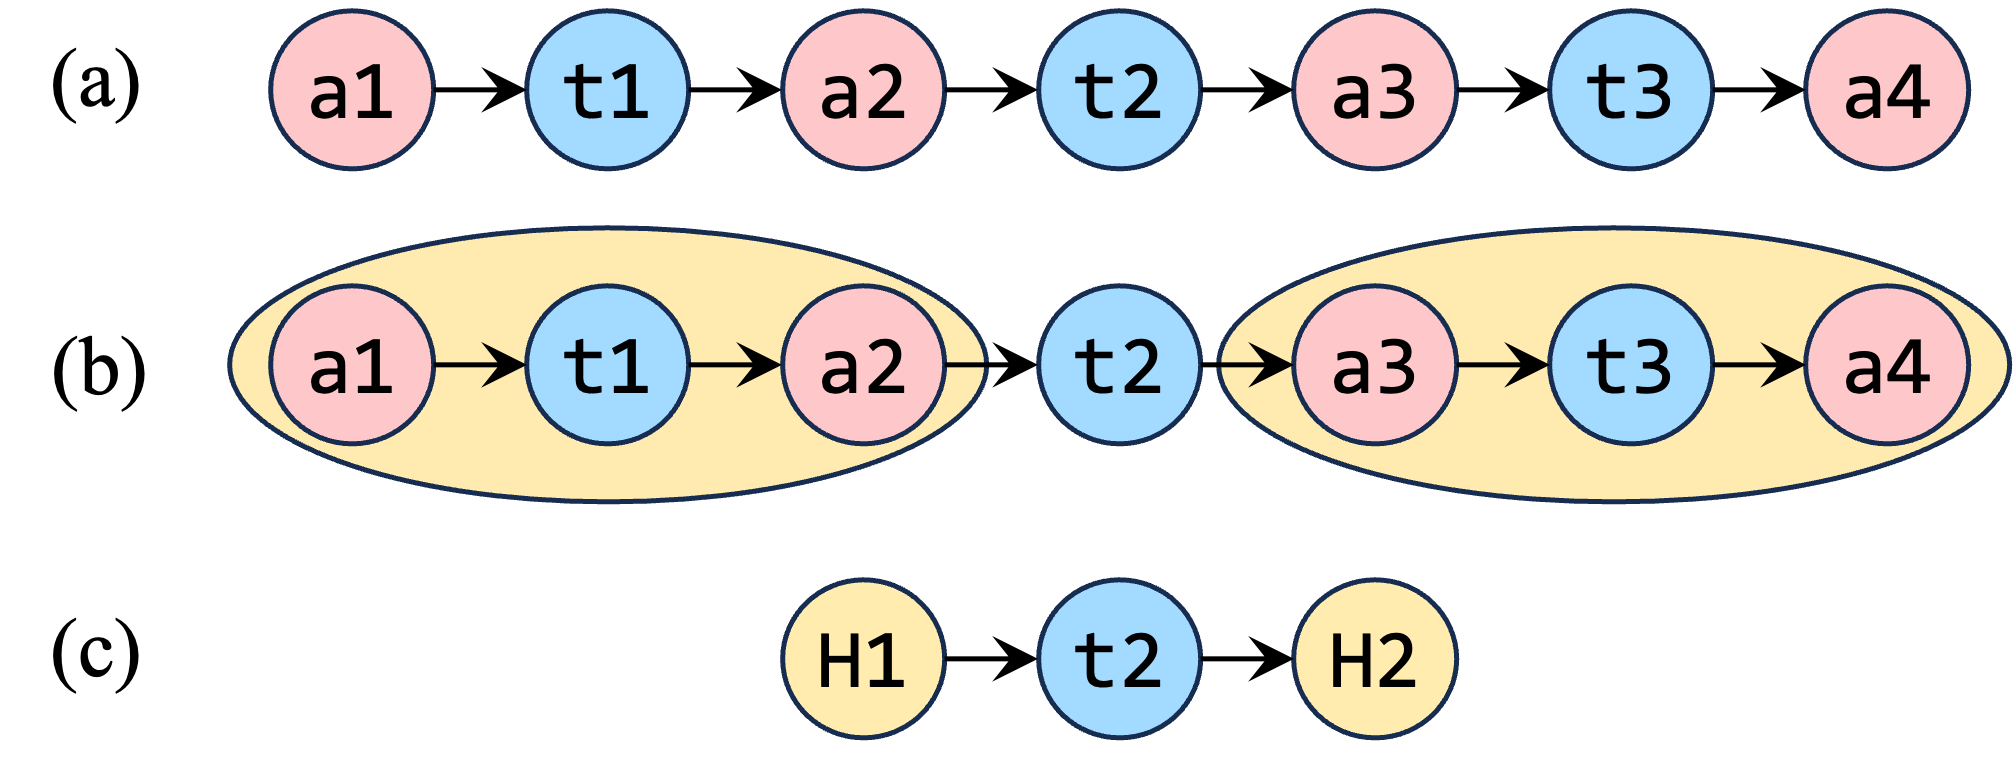
\includegraphics[width=0.7\linewidth]{figures/intuition-example.png}
    \caption{Decomposing a 3-hop query into parallel one-hop operators 
    ($H_1$, $H_2$) and a residual 3-way join, reducing a 7-way join tree 
    to a 3-way join tree.}
    \label{fig:intuition}
\end{figure}

\noindent\textbf{Why this outperforms applying \wei directly.}
Treating the query as a flat 7-way join and feeding it to \wei is 
correct but wasteful. Their scheme fails to
exploit bidirectional edges, cannot fuse predicates into the traversal, 
and processes the full join tree sequentially --- each parent-child pair 
in the tree requires six oblivious sorts (a total of XX for the 7-way join).
Worse, when predicates are present, \wei 
applies filtering only after the join materializes its output, exposing the 
unfiltered intermediate size to the adversary. \system avoids all of this: 
the one-hop operator collapses a three-way join into a single sort, the 
decomposer eliminates join depth by running independent hops in parallel, 
and in-place filtering ensures the adversary learns only the base table 
sizes, the query structure, and the final filtered result size.

\system's query processing engine comprises two components beyond \wei: 
the \onehop operator (Section~\ref{sec:onehop}), which implements the 
efficient single-sort traversal with in-place filtering, and the query 
decomposer (Section~\ref{sec:decomposition}), which identifies independent 
one-hop patterns and rewrites multi-hop queries into parallelizable 
components feeding a reduced residual join.